%
\begin{figure}%
  \def\frac{0.24}
  On Fetch Reach\\
  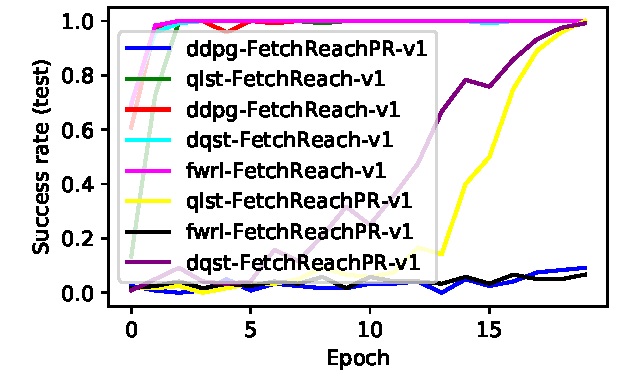
\includegraphics[width=\frac\columnwidth]{media/res/245b3c4-ce781a70-FetchReachPR-v1-fwrl-future-her_fwrl_path_reward/test/success_rate.pdf}%
  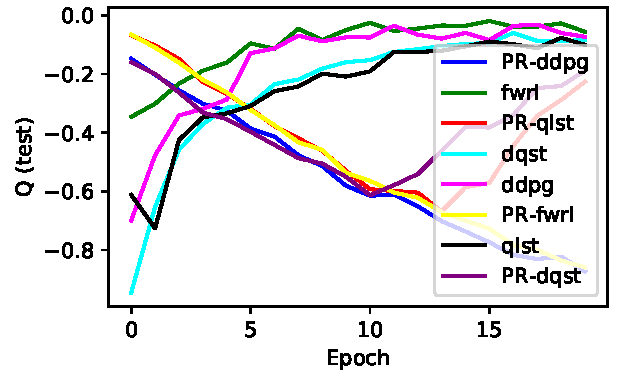
\includegraphics[width=\frac\columnwidth]{media/res/245b3c4-ce781a70-FetchReachPR-v1-fwrl-future-her_fwrl_path_reward/test/mean_Q.pdf}%
  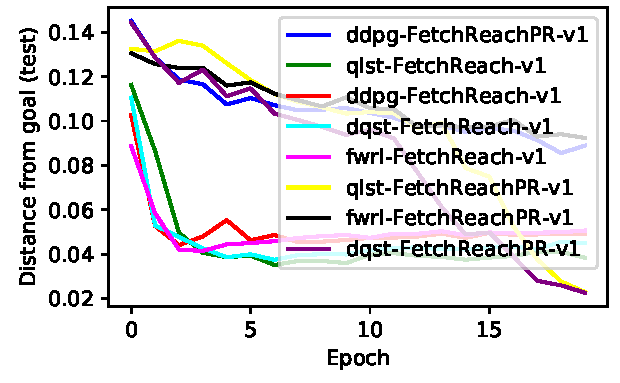
\includegraphics[width=\frac\columnwidth]{media/res/245b3c4-ce781a70-FetchReachPR-v1-fwrl-future-her_fwrl_path_reward/test/ag_g_dist.pdf}%
  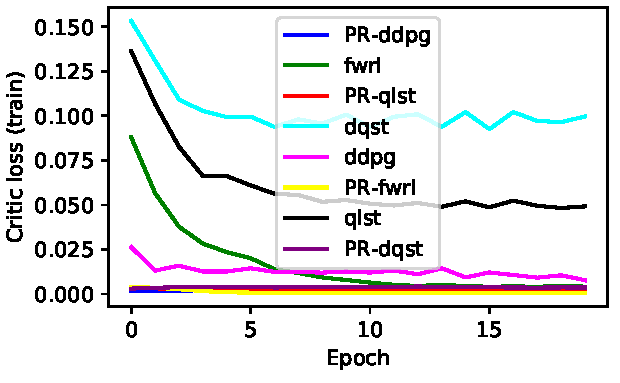
\includegraphics[width=\frac\columnwidth]{media/res/245b3c4-ce781a70-FetchReachPR-v1-fwrl-future-her_fwrl_path_reward/train/critic_loss.pdf}\\
  On Fetch Push\\
  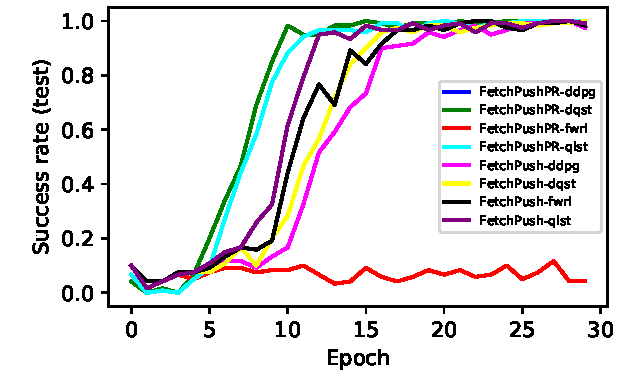
\includegraphics[width=\frac\columnwidth]{./media/res/be0910c-her_fwrl_path_reward-FetchPushPR-v1-fwrl/test/success_rate.pdf}%
  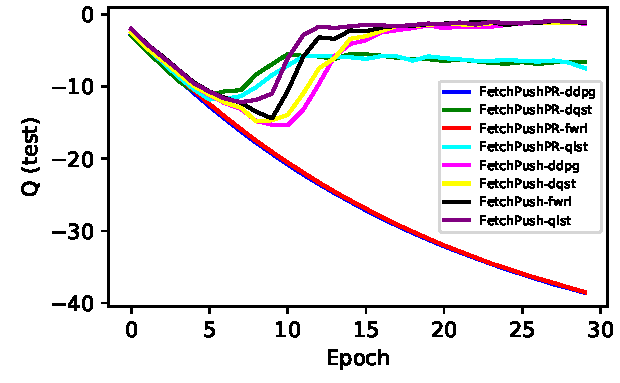
\includegraphics[width=\frac\columnwidth]{./media/res/be0910c-her_fwrl_path_reward-FetchPushPR-v1-fwrl/test/mean_Q.pdf}%
  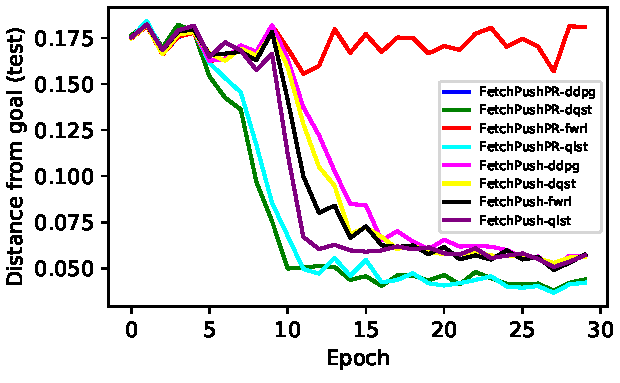
\includegraphics[width=\frac\columnwidth]{./media/res/be0910c-her_fwrl_path_reward-FetchPushPR-v1-fwrl/test/ag_g_dist.pdf}%
  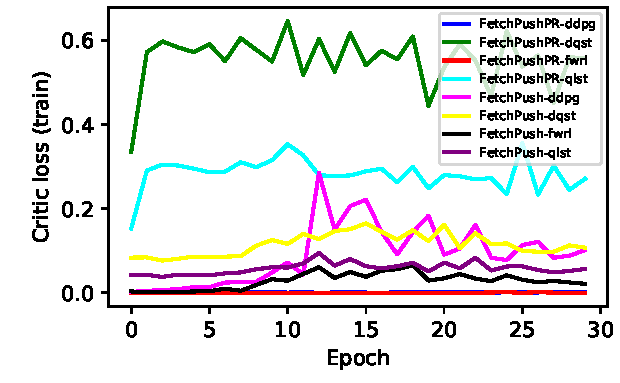
\includegraphics[width=\frac\columnwidth]{./media/res/be0910c-her_fwrl_path_reward-FetchPushPR-v1-fwrl/train/critic_loss.pdf}\\
  On Fetch Slide\\
  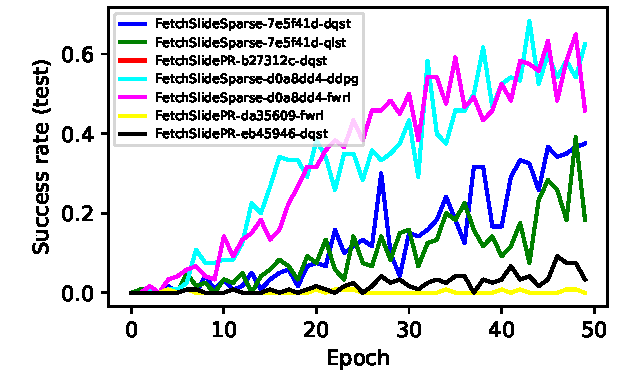
\includegraphics[width=\frac\columnwidth]{./media/res/eb45946-path_reward-FetchSlidePR-v1-dqst/test/success_rate.pdf}%
  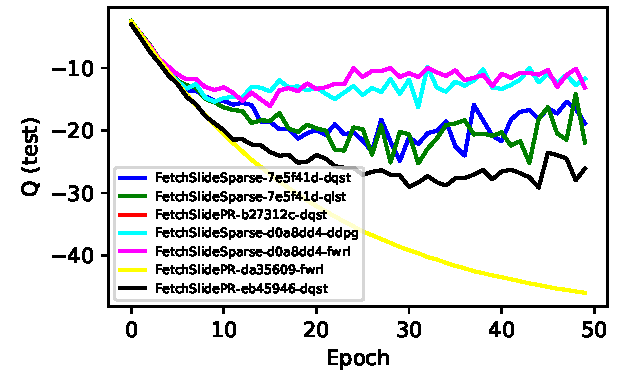
\includegraphics[width=\frac\columnwidth]{./media/res/eb45946-path_reward-FetchSlidePR-v1-dqst/test/mean_Q.pdf}%
  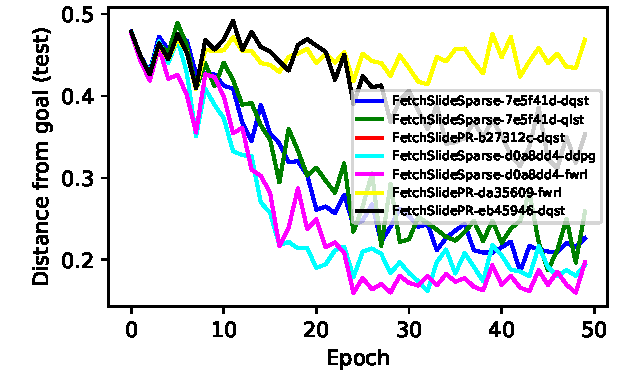
\includegraphics[width=\frac\columnwidth]{./media/res/eb45946-path_reward-FetchSlidePR-v1-dqst/test/ag_g_dist.pdf}%
  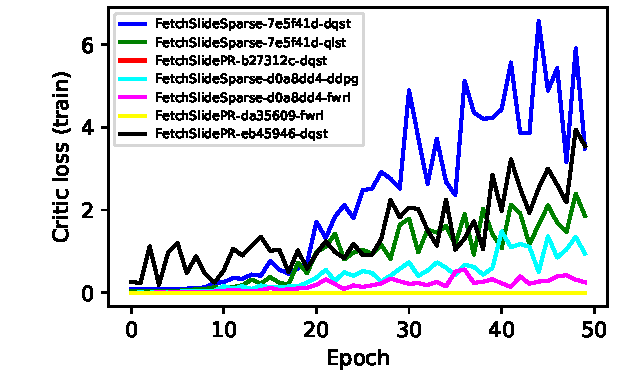
\includegraphics[width=\frac\columnwidth]{./media/res/eb45946-path_reward-FetchSlidePR-v1-dqst/train/critic_loss.pdf}\\
  On Fetch Pick And Place\\
  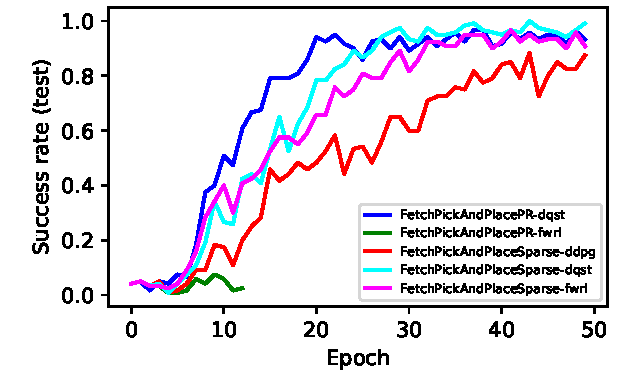
\includegraphics[width=\frac\columnwidth]{./media/res/d5cefef-path_reward-FetchPickAndPlacePR-v1-dqst/test/success_rate.pdf}%
  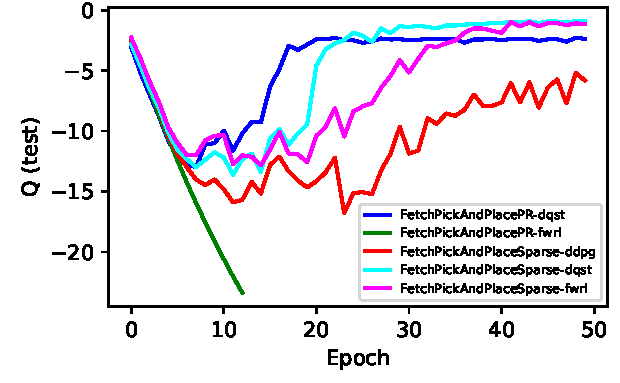
\includegraphics[width=\frac\columnwidth]{./media/res/d5cefef-path_reward-FetchPickAndPlacePR-v1-dqst/test/mean_Q.pdf}%
  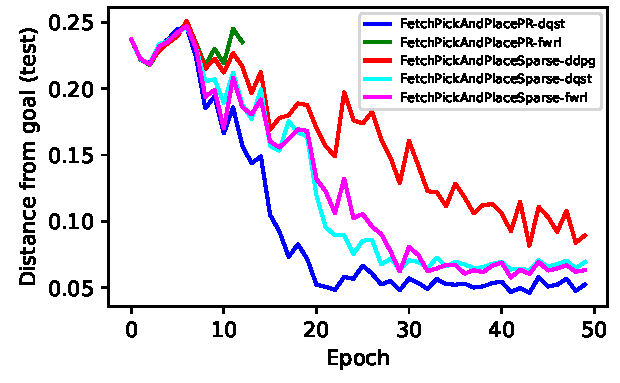
\includegraphics[width=\frac\columnwidth]{./media/res/d5cefef-path_reward-FetchPickAndPlacePR-v1-dqst/test/ag_g_dist.pdf}%
  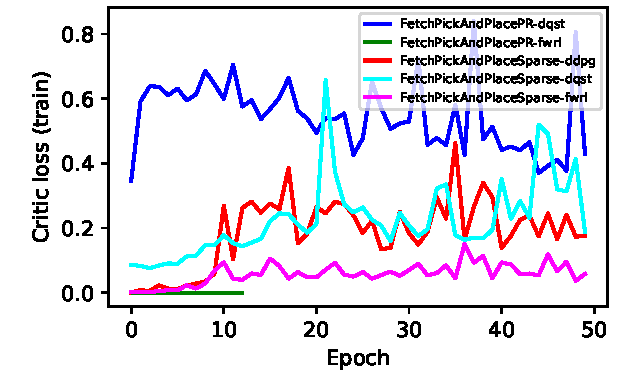
\includegraphics[width=\frac\columnwidth]{./media/res/d5cefef-path_reward-FetchPickAndPlacePR-v1-dqst/train/critic_loss.pdf}\\
  On Hand Reach \\
  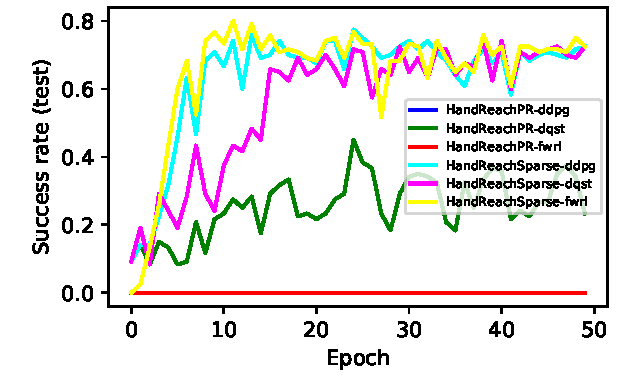
\includegraphics[width=\frac\columnwidth]{./media/res/d5cefef-path_reward-HandReachPR-v0-dqst/test/success_rate.pdf}%
  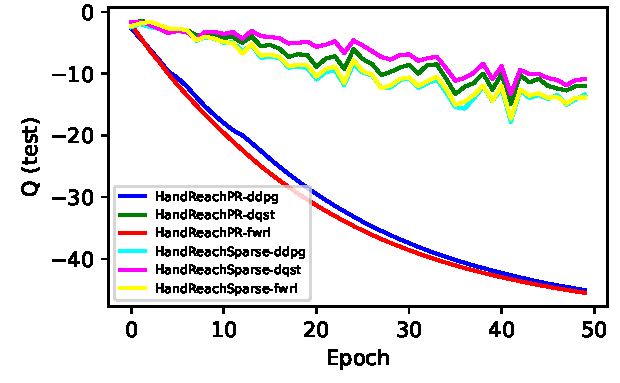
\includegraphics[width=\frac\columnwidth]{./media/res/d5cefef-path_reward-HandReachPR-v0-dqst/test/mean_Q.pdf}%
  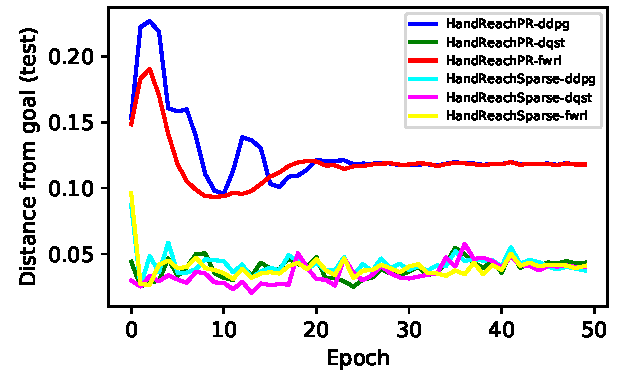
\includegraphics[width=\frac\columnwidth]{./media/res/d5cefef-path_reward-HandReachPR-v0-dqst/test/ag_g_dist.pdf}%
  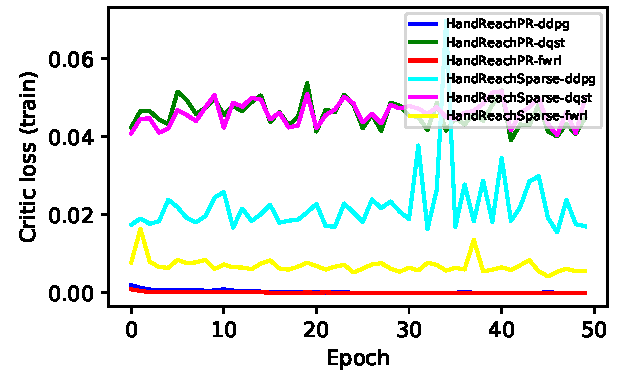
\includegraphics[width=\frac\columnwidth]{./media/res/d5cefef-path_reward-HandReachPR-v0-dqst/train/critic_loss.pdf}\\
  \label{fig:path-reward-1}%
  \caption{Effect of path reward on convergence in case of different loss
    functions on FetchReach. With path reward on PR-dqst
    ($\LossDDPG$ + $\LossStep$)
    and PR-qlst
    ($\LossDDPG$ + $\LossStep$ + $\LossLo$ + $\LossUp$), are able achieve high
    success rate and even that takes longer than usual. Out of the two PR-dqst
    does better. The terms with PR use path-rewards and hence less computation
    by avoid recomputation of reward function. It is interesting that PR-dqst
    and PR-qlst reach closer in terms of distance from goal probably because of
    absence of threshold.}%
\end{figure}%
% 

\begin{figure}
  \def\frac{0.32}
    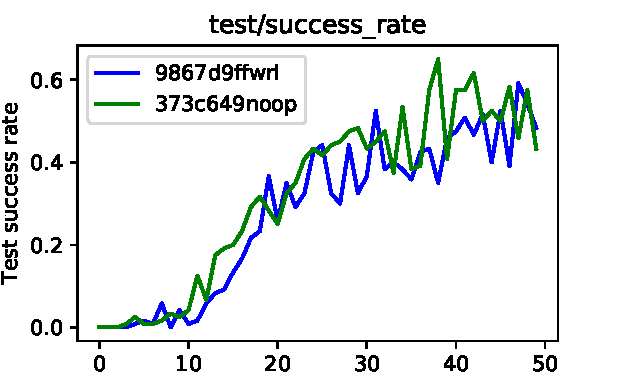
\includegraphics[width=\frac\columnwidth]{media/res/373c649_FetchSlide-v1-noop/test/success_rate.pdf}%
    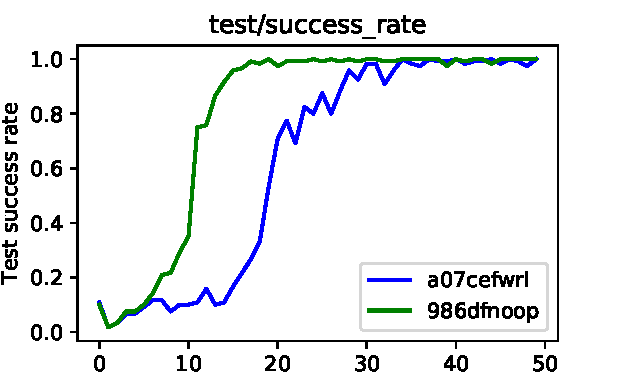
\includegraphics[width=\frac\columnwidth]{media/res/a077c9e_FetchPush-v1-fwrl/test/success_rate.pdf}%
    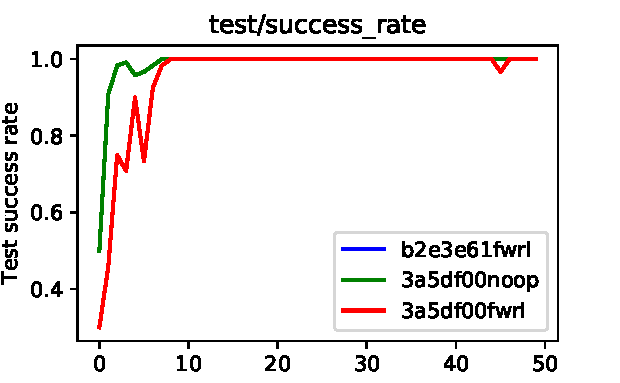
\includegraphics[width=\frac\columnwidth]{media/res/3a5df00_FetchReach-v1-fwrl/test/success_rate.pdf}\\
    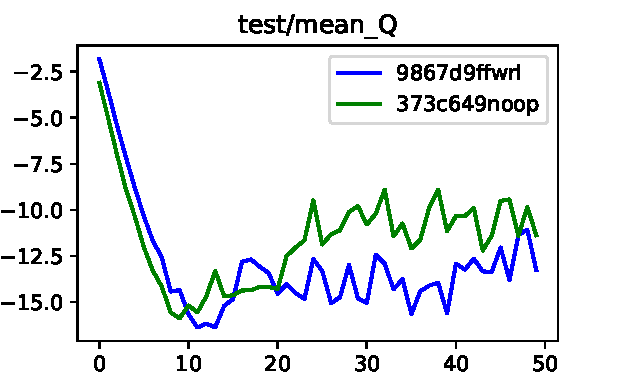
\includegraphics[width=\frac\columnwidth]{media/res/373c649_FetchSlide-v1-noop/test/mean_Q.pdf}%
    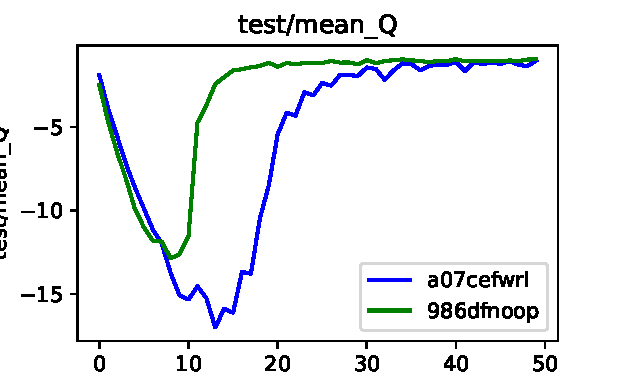
\includegraphics[width=\frac\columnwidth]{media/res/a077c9e_FetchPush-v1-fwrl/test/mean_Q.pdf}%
    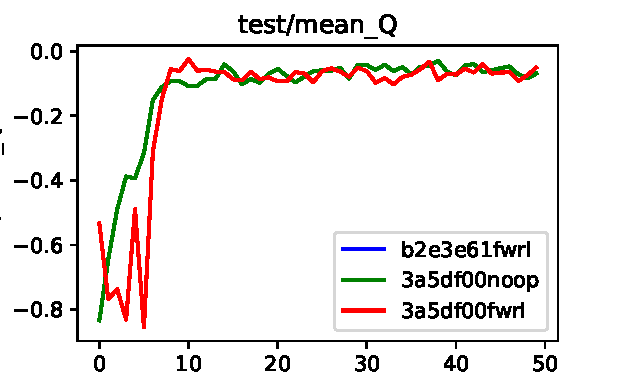
\includegraphics[width=\frac\columnwidth]{media/res/3a5df00_FetchReach-v1-fwrl/test/mean_Q.pdf}
    \caption{fwrl = Floyd Warshall ($=\Loss_{\text{ddpg}} +
      \Loss_{\text{upper}}$) with HER sampling;
      noop = DDPG ($=\Loss_{\text{ddpg}}$)with HER sampling.
  Test success rate and Mean Q on (1) Fetch-Slide, (2) Fetch-Push and (3)
  Fetch-Reach task. fwrl does consistently worse than HER.}
    \label{fig:fetch-slide-success}
\end{figure}


%
\begin{figure}%
  \def\frac{0.24}
  With HER sampling:\\
  \includegraphics[width=\frac\columnwidth]{media/res/3a90344-FetchReach-v1-stepfwrl-future/test/success_rate.pdf}%
  \includegraphics[width=\frac\columnwidth]{media/res/3a90344-FetchReach-v1-stepfwrl-future/test/mean_Q.pdf}%
  \includegraphics[width=\frac\columnwidth]{media/res/3a90344-FetchReach-v1-stepfwrl-future/train/critic_loss.pdf}%
  \includegraphics[width=\frac\columnwidth]{media/res/3a90344-FetchReach-v1-stepfwrl-future/train/critic_addnl_loss.pdf}\\
  Without HER sampling:\\
  \includegraphics[width=\frac\columnwidth]{media/res/d047a03-FetchReach-v1-stepfwrl-none/test/success_rate.pdf}%
  \includegraphics[width=\frac\columnwidth]{media/res/d047a03-FetchReach-v1-stepfwrl-none/test/mean_Q.pdf}%
  \includegraphics[width=\frac\columnwidth]{media/res/d047a03-FetchReach-v1-stepfwrl-none/train/critic_loss.pdf}%
  \includegraphics[width=\frac\columnwidth]{media/res/d047a03-FetchReach-v1-stepfwrl-none/train/critic_addnl_loss.pdf}\\
Using both upper and lower bound in FWRL\\
  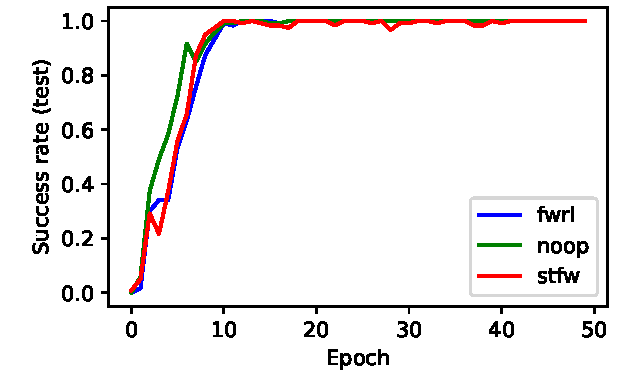
\includegraphics[width=\frac\columnwidth]{media/res/f0d4cfa-FetchReach-v1-stfw-none/test/success_rate.pdf}%
  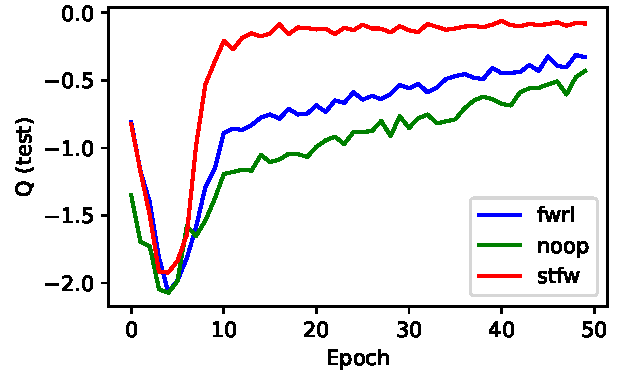
\includegraphics[width=\frac\columnwidth]{media/res/f0d4cfa-FetchReach-v1-stfw-none/test/mean_Q.pdf}%
  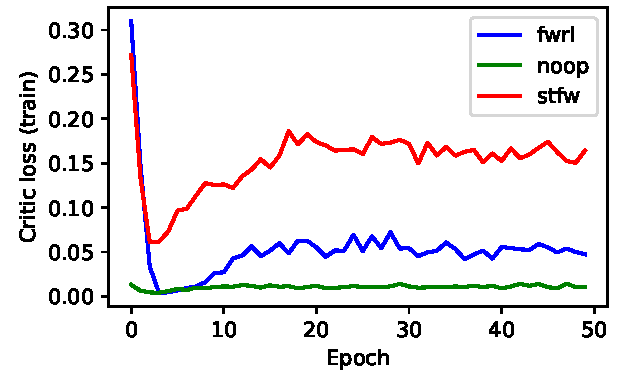
\includegraphics[width=\frac\columnwidth]{media/res/f0d4cfa-FetchReach-v1-stfw-none/train/critic_loss.pdf}%
  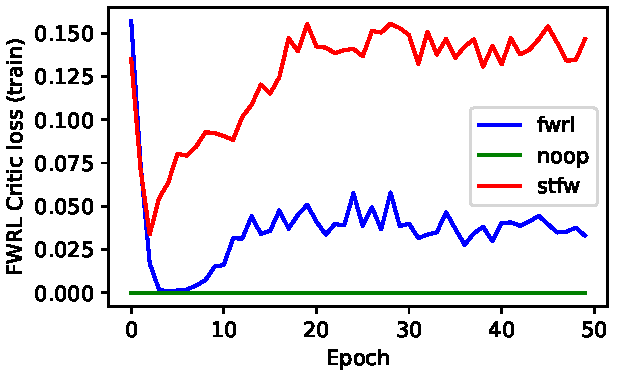
\includegraphics[width=\frac\columnwidth]{media/res/f0d4cfa-FetchReach-v1-stfw-none/train/critic_addnl_loss.pdf}\\
  \caption{
    stepfwrl = DDPG loss $\Loss_{\text{ddpg}}$ + Step loss $\Loss_{\text{step}}$
    + FWRL constraints $\Loss_{\text{upper}} + \Loss_{\text{lower}}$, noop =
    DDPG loss $\Loss_{\text{ddpg}}$  + HER
    sampling, fwrl = DDPG Loss $\Loss_{\text{ddpg}}$ + FWRL constraints $\Loss_{\text{upper}} + \Loss_{\text{lower}}$.
    All experiments on Fetch-Reach task.
  }%
  \label{fig:fwrl-stepfwrl-noop-FetchReach}%
\end{figure}%
% 

%
\begin{figure}%
  \def\frac{0.24}
  With HER sampling\\
  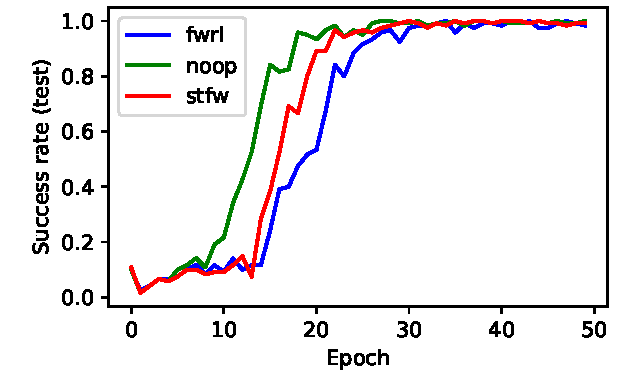
\includegraphics[width=\frac\columnwidth]{media/res/ea0e35b-FetchPush-v1-stfw-future/test/success_rate.pdf}%
  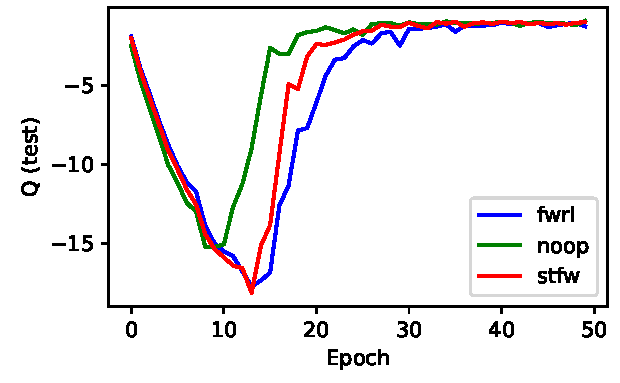
\includegraphics[width=\frac\columnwidth]{media/res/ea0e35b-FetchPush-v1-stfw-future/test/mean_Q.pdf}%
  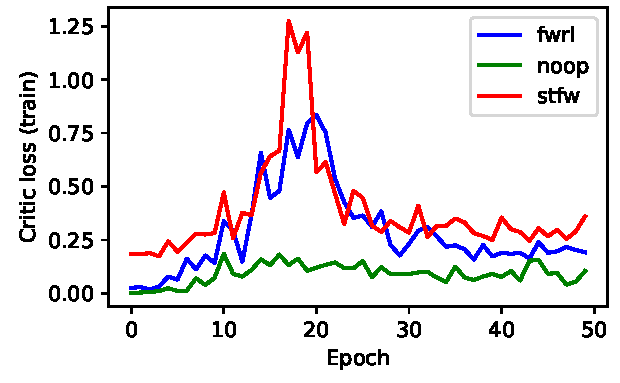
\includegraphics[width=\frac\columnwidth]{media/res/ea0e35b-FetchPush-v1-stfw-future/train/critic_loss.pdf}%
  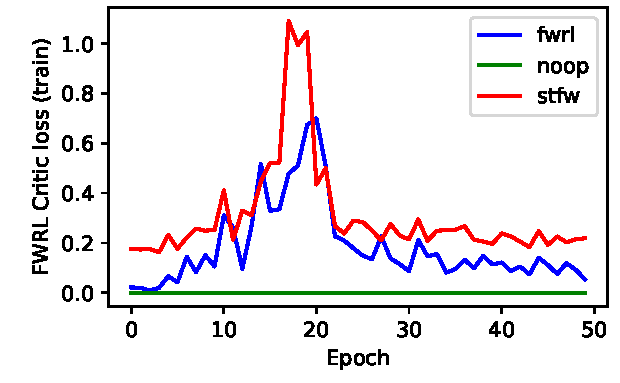
\includegraphics[width=\frac\columnwidth]{media/res/ea0e35b-FetchPush-v1-stfw-future/train/critic_addnl_loss.pdf}\\
  Without HER sampling\\
  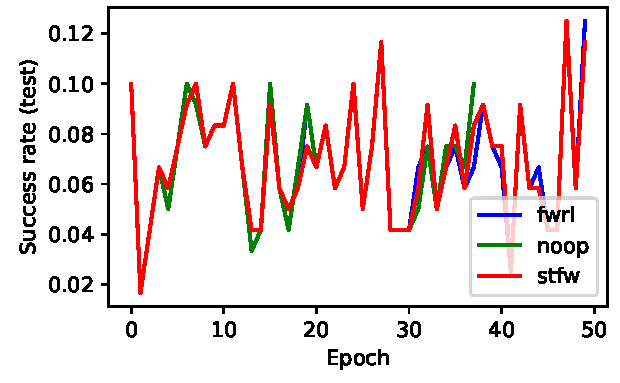
\includegraphics[width=\frac\columnwidth]{media/res/ea0e35b-FetchPush-v1-stfw-none/test/success_rate.pdf}%
  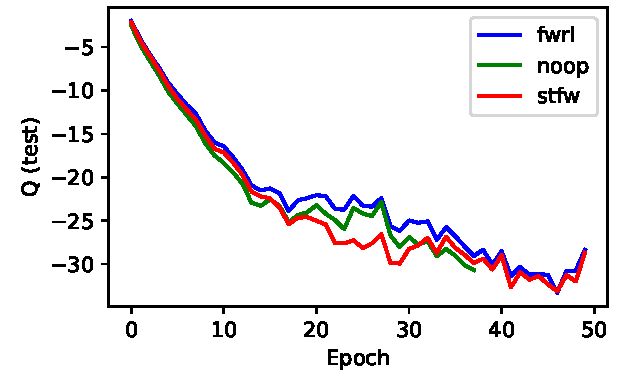
\includegraphics[width=\frac\columnwidth]{media/res/ea0e35b-FetchPush-v1-stfw-none/test/mean_Q.pdf}%
  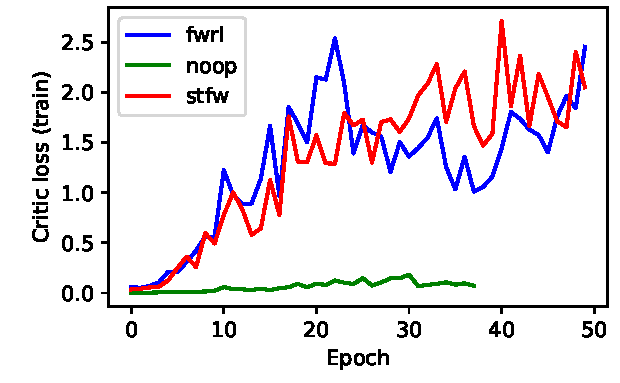
\includegraphics[width=\frac\columnwidth]{media/res/ea0e35b-FetchPush-v1-stfw-none/train/critic_loss.pdf}%
  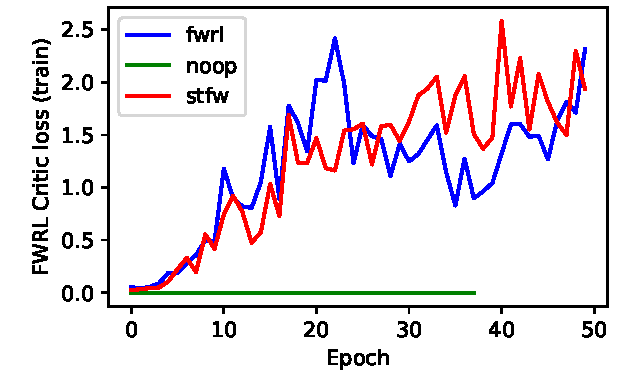
\includegraphics[width=\frac\columnwidth]{media/res/ea0e35b-FetchPush-v1-stfw-none/train/critic_addnl_loss.pdf}%
  \caption{stepfwrl = DDPG loss $\Loss_{\text{ddpg}}$ + Step loss $\Loss_{\text{step}}$
    + FWRL constraints $\Loss_{\text{upper}} + \Loss_{\text{lower}}$, noop =
    DDPG loss $\Loss_{\text{ddpg}}$  + HER
    sampling, fwrl = DDPG Loss $\Loss_{\text{ddpg}}$ + FWRL constraints $\Loss_{\text{upper}} + \Loss_{\text{lower}}$.
    All experiments on Fetch-Push}
  \label{fig:loss-func-fetch-push}
\end{figure}
%

%
\begin{figure}
  \def\frac{0.32}
Loss function breakdown without HER sampling on Fetch Push\\
  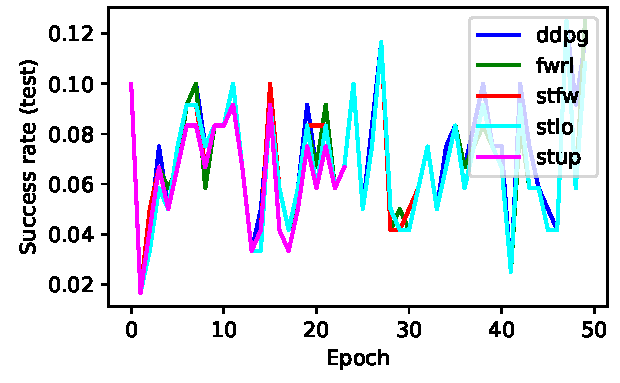
\includegraphics[width=\frac\columnwidth]{media/res/f84daa7-FetchPush-v1-stfw-none/test/success_rate.pdf}%
  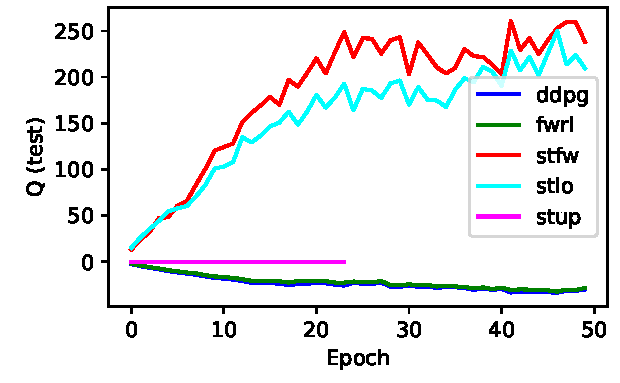
\includegraphics[width=\frac\columnwidth]{media/res/f84daa7-FetchPush-v1-stfw-none/test/mean_Q.pdf}%
  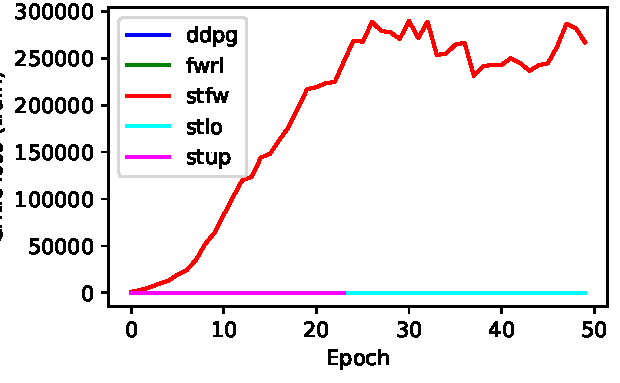
\includegraphics[width=\frac\columnwidth]{media/res/f84daa7-FetchPush-v1-stfw-none/train/critic_loss.pdf}\\
Loss function breakdown with HER sampling on Fetch Push\\
  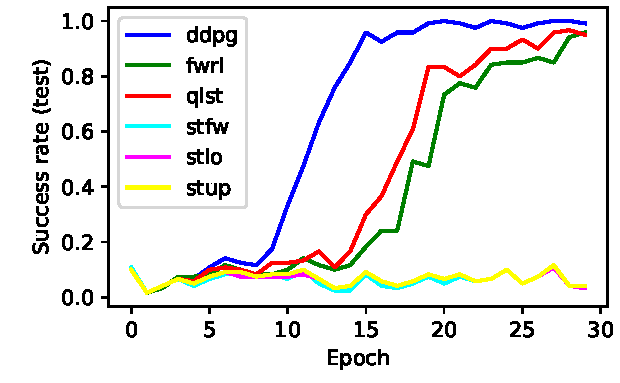
\includegraphics[width=\frac\columnwidth]{media/res/3f1eafe-FetchPush-v1-stfw-future/test/success_rate.pdf}%
  \includegraphics[width=\frac\columnwidth]{media/res/3f1eafe-FetchPush-v1-stfw-future/test/mean_Q.pdf}%
  \includegraphics[width=\frac\columnwidth]{media/res/3f1eafe-FetchPush-v1-stfw-future/train/critic_loss.pdf}%
  \caption{
    Fetch Push results. Loss function changes do no seem to make a difference.
    There are four parts to the loss function (1) DDPG Loss $\Loss_{\text{ddpg}}$ ,
    (2) Step loss$\Loss_{\text{step}}$,  
    (3) Lower bound $\Loss_{\text{lower}}$ and
    (4) Upper bound $\Loss_{\text{upper}}$ .
    ddpg = $\Loss_{\text{ddpg}}$,
    dqst = $\Loss_{\text{ddpg}}$ + $\Loss_{\text{step}}$,
    fwrl = $\Loss_{\text{ddpg}}$ + $\Loss_{\text{lower}}$ +
    $\Loss_{\text{upper}}$,
    qlst = $\Loss_{\text{ddpg}}$ + $\Loss_{\text{step}}$ + $\Loss_{\text{lower}}$ + $\Loss_{\text{upper}}$.
    stfw = $\Loss_{\text{step}}$ + $\Loss_{\text{lower}}$ + $\Loss_{\text{upper}}$,
    stlo = $\Loss_{\text{step}}$ + $\Loss_{\text{lower}}$,
    stup = $\Loss_{\text{step}}$ + $\Loss_{\text{upper}}$.
    Success rate is the fraction of times the agent reaches the goal. Q(test) is
    the estimated cumulative reward by the network. Critic loss is the total
    loss plotted during training.
    Because stfw, stlo, stup fail to succeed, we infer that the $\Loss_{\text{ddpg}}$ DDPG loss is
    critical for making the algorithm work. Since the qlst works better than
    fwrl, we infer that $\Loss_{\text{step}}$ Step loss is also important.
    only.
    Since there is slight improvement in dqst over ddpg, this means
    $\Loss_{\text{step}}$ really helps. dqst did not run fully but it shows
    promise (I need to fix a bug).
    But why does the loss for stfw keep rising? Does it mean that the SGD is not
    able to optimize the loss gradients in the right direction?
  }%
  \label{fig:fwrl-stepfwrl-noop-FetchPush}%
\end{figure}%
% 

%
\begin{figure}
  \def\frac{0.32}
  On Fetch Push\\
  \includegraphics[width=\frac\columnwidth]{media/res/38f4625-FetchPush-v1-fwrl-future/test/success_rate.pdf}%
  \includegraphics[width=\frac\columnwidth]{media/res/38f4625-FetchPush-v1-fwrl-future/test/mean_Q.pdf}%
  \includegraphics[width=\frac\columnwidth]{media/res/38f4625-FetchPush-v1-fwrl-future/train/critic_loss.pdf}\\
  On Fetch Reach\\
  \includegraphics[width=\frac\columnwidth]{media/res/38f4625-FetchReach-v1-fwrl-future/test/success_rate.pdf}%
  \includegraphics[width=\frac\columnwidth]{media/res/38f4625-FetchReach-v1-fwrl-future/test/mean_Q.pdf}%
  \includegraphics[width=\frac\columnwidth]{media/res/38f4625-FetchReach-v1-fwrl-future/train/critic_loss.pdf}\\
  On Fetch Slide\\
  \includegraphics[width=\frac\columnwidth]{media/res/38f4625-FetchSlide-v1-fwrl-future/test/success_rate.pdf}%
  \includegraphics[width=\frac\columnwidth]{media/res/38f4625-FetchSlide-v1-fwrl-future/test/mean_Q.pdf}%
  \includegraphics[width=\frac\columnwidth]{media/res/38f4625-FetchSlide-v1-fwrl-future/train/critic_loss.pdf}%
  On Fetch Pick and Place\\
  \includegraphics[width=\frac\columnwidth]{media/res/38f4625-FetchPickAndPlace-v1-fwrl-future/test/success_rate.pdf}%
  \includegraphics[width=\frac\columnwidth]{media/res/38f4625-FetchPickAndPlace-v1-fwrl-future/test/mean_Q.pdf}%
  \includegraphics[width=\frac\columnwidth]{media/res/38f4625-FetchPickAndPlace-v1-fwrl-future/train/critic_loss.pdf}%
  On HandReach\\
  \includegraphics[width=\frac\columnwidth]{media/res/38f4625-92450888-HandReach-v0-fwrl-future/test/success_rate.pdf}%
  \includegraphics[width=\frac\columnwidth]{media/res/38f4625-92450888-HandReach-v0-fwrl-future/test/mean_Q.pdf}%
  \includegraphics[width=\frac\columnwidth]{media/res/38f4625-92450888-HandReach-v0-fwrl-future/train/critic_loss.pdf}%
  \caption{
    Fetch results. Loss function changes do no seem to make a difference.
    There are four parts to the loss function (1) DDPG Loss $\LossDDPG$ ,
    (2) Step loss$\LossStep$,  
    (3) Lower bound $\LossLo$ and
    (4) Upper bound $\LossUp$ .
    ddpg = $\LossDDPG$,
    dqst = $\LossDDPG$ + $\LossStep$,
    fwrl = $\LossDDPG$ + $\LossLo$ +
    $\LossUp$,
    qlst = $\LossDDPG$ + $\LossStep$ + $\LossLo$ + $\LossUp$,
    dqte = $\LossDDPG$ + $\LossTrieq$,
    qste = $\LossDDPG$ + $\LossStep$ + $\LossTrieq$.
    Success rate is the fraction of times the agent reaches the goal. Q(test) is
    the estimated cumulative reward by the network. Critic loss is the total
    loss plotted during training.
    Because stfw, stlo, stup fail to succeed, we infer that the $\LossDDPG$ DDPG loss is
    critical for making the algorithm work. Since the qlst works better than
    fwrl, we infer that $\LossStep$ Step loss is also important.
    only.
    Since there is slight improvement in dqst over ddpg, this means
    $\LossStep$ really helps. dqst did not run fully but it shows
    promise (I need to fix a bug).
    But why does the loss for stfw keep rising? Does it mean that the SGD is not
    able to optimize the loss gradients in the right direction?
  }%
  \label{fig:fwrl-stepfwrl-noop-FetchPush}%
\end{figure}%
% 

%
\begin{figure}%
  \def\frac{0.25}
  \includegraphics[width=\frac\columnwidth]{media/res/3d07a6e-FetchReachPR-v1-fwrl-future/test/success_rate.pdf}%
  \includegraphics[width=\frac\columnwidth]{media/res/3d07a6e-FetchReachPR-v1-fwrl-future/test/mean_Q.pdf}%
  \includegraphics[width=\frac\columnwidth]{media/res/3d07a6e-FetchReachPR-v1-fwrl-future/test/ag_g_dist.pdf}%
  \includegraphics[width=\frac\columnwidth]{media/res/3d07a6e-FetchReachPR-v1-fwrl-future/train/critic_loss.pdf}%
  \label{fig:path-rewards}%
  \caption{Experiment to see the effect of only path rewards on loss terms. We
    did not include a step term which becomes very important in this case.}%
\end{figure}%
% 

%
\begin{figure}%
  \def\frac{0.24}
  \includegraphics[width=\frac\columnwidth]{./media/res/04a8fc6-814a3d24-FetchSlide-v1-fwrl-future/test/success_rate.pdf}%
  \includegraphics[width=\frac\columnwidth]{./media/res/04a8fc6-814a3d24-FetchSlide-v1-fwrl-future/test/mean_Q.pdf}%
  \includegraphics[width=\frac\columnwidth]{./media/res/04a8fc6-814a3d24-FetchSlide-v1-fwrl-future/test/ag_g_dist.pdf}%
  \includegraphics[width=\frac\columnwidth]{./media/res/04a8fc6-814a3d24-FetchSlide-v1-fwrl-future/train/critic_loss.pdf}%
  \label{fig:loss-term-weights}%
  \caption{Effect of weighted combination of loss terms on FetchSlide. The three
  loss terms being weighed in order are $[\LossDDPG, \LossLo, \LossUp]$}%
\end{figure}%
% 
We compared weighted combination of loss terms

%
\begin{figure}%
  \def\frac{0.24}
  \includegraphics[width=\frac\columnwidth]{media/res/d249d2d-c9bfa98b-FetchPush-v1-fwrl-future/test/success_rate.pdf}%
  \includegraphics[width=\frac\columnwidth]{media/res/d249d2d-c9bfa98b-FetchPush-v1-fwrl-future/test/mean_Q.pdf}%
  \includegraphics[width=\frac\columnwidth]{media/res/d249d2d-c9bfa98b-FetchPush-v1-fwrl-future/test/ag_g_dist.pdf}%
  \includegraphics[width=\frac\columnwidth]{media/res/d249d2d-c9bfa98b-FetchPush-v1-fwrl-future/train/critic_loss.pdf}%
  \label{fig:middle-vs-uniform}%
  \caption{Effect of choosing the intermediate sample in the \emph{middle} of the
    trajectory vs \emph{uniform}ly random in the trajectory on FetchPush}%
\end{figure}%
% 

%
\begin{figure}%
  \includegraphics[width=\columnwidth]{./media/res/eb45946-path_reward-FetchSlidePR-v1-dqst/test/success_rate.pdf}%
  \label{fig:}%
  \caption{Effect of path rewards on FetchSlide}%
\end{figure}%
% 

%\subsection{Unanswered questions and things to try}
%
%\subsubsection{FWRL specific sampling}
%Right now the shuffle step in the algorithm is totally random and probably
%introduces more noise in the algorithm than it helps. A modification of HER
%sampling would sampling three time steps from the trajectory (single episode)
%$t_1 > t_2 > t_3$ and use $t_2$ as the intermediate state for
%$\LossUp$ and $\LossLo$.
%
%
%\subsubsection{Why is any loss term with upper/lower worse?}
%This is probably answered by  the above section but what are the other
%explanations. The total ``Critic loss'' is increasing for stfw
%($=\LossStep$ + $\LossLo$ + $\LossUp$),
%which seems to say that with $\LossDDPG$, it is hard to optimize the functions.
%
%
%\subsection{Is it still a contribution if the upper and lower bounds do not
%  improve the results?}
%Can we claim that this alternative formulation is new and more principled than HER?